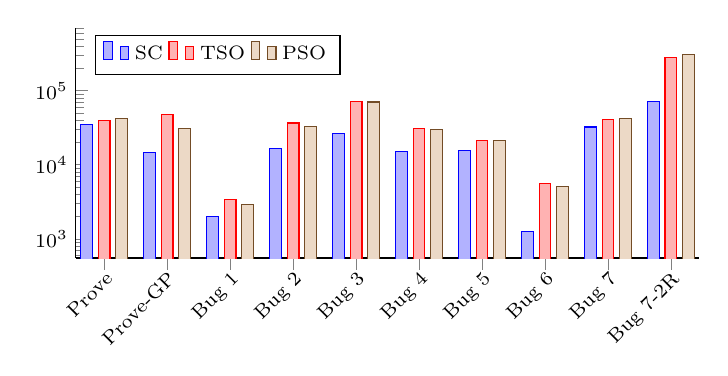
\begin{tikzpicture}
\scriptsize
\begin{axis}[
  ybar,
  bar width=0.15cm,
  height=4.5cm,
  width=9.5cm,
  axis lines*=left, % remove lines in the background
  ymode=log,
  %ylabel=Total runtime (seconds),
  symbolic x coords={Prove, Prove-GP, Bug 1, Bug 2, Bug 3, 
                     Bug 4, Bug 5, Bug 6, Bug 7, Bug 7-2R,
                    },
  xtick=data,
  %nodes near coords, % numbers displayed above the bars
  %every node near coord/.append style={font=\small, rotate=90, anchor=west},
  xticklabel style={
    inner sep=0pt,
    anchor=north east,
    rotate=45
  },
  %enlargelimits=0.15,
  enlarge y limits=0.15, % space relative to the height of the plot
  enlarge x limits=0.05, % space relative to the width of the plot
  legend style={
    %anchor=north, at={(0.5, -0.9)}, % legend location
    legend pos=north west,
    legend columns=-1,
    font=\scriptsize},
]

\addplot % SC
  coordinates {(Prove, 34570.5) (Prove-GP, 14698.4)
               (Bug 1, 2002.53) (Bug 2, 16644.8) (Bug 3, 26716.8)
               (Bug 4, 15231.3) (Bug 5, 15490.8) (Bug 6, 1255.06)
               (Bug 7, 32373.1) (Bug 7-2R, 70822.7)
              };

\addplot % TSO 
  coordinates {(Prove, 39820.1) (Prove-GP, 47643.6)
               (Bug 1, 3360.95) (Bug 2, 36608.3) (Bug 3, 71708.5)
               (Bug 4, 30599.2) (Bug 5, 21550.4) (Bug 6, 5608.83)
               (Bug 7, 40667.7) (Bug 7-2R, 283950)
              };


\addplot % PSO
  coordinates {(Prove, 41754.8) (Prove-GP, 31002.2)
               (Bug 1, 2902.64) (Bug 2, 32616.8) (Bug 3, 70477.1)
               (Bug 4, 30355) (Bug 5, 21296.9) (Bug 6, 5040.28)
               (Bug 7, 42226) (Bug 7-2R, 306133)
              };

\legend{SC, TSO, PSO}
\end{axis}
\end{tikzpicture}
